In dit hoofdstuk worden de verschillende lasten van de moonrover berekend. In de formules word er een hellingshoek aangehouden van 0 graden. De beschreven formules zijn allemaal voor 1 wiel. Voor de gehele moonrover zal dit dus x4 moeten. In de afbeeldingen is ook te zien hoe de eigenschappen zich gedragen onder diverse hellingshoeken.

\subsection{Rollast}
    Rollast is de last die minimaal overwonnen moet worden om een wiel te laten draaien. Dit verschilt ook onder welke hellingshoek de moonrover staat. In afbeelding \ref{fig:birds} is te zien hoe de rolllast verandert onder diverse hellingshoeken.

    \begin{figure}[H]
        \centering
        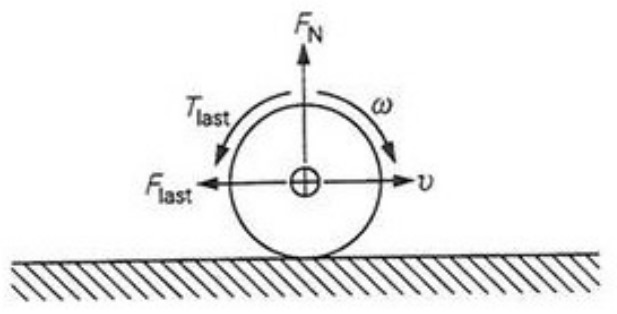
\includegraphics[scale=0.5]{Rolweerstand.jpg}
        \caption{rollast krachten}
    \end{figure}

    \begin{multicols}{2}
        \textbf{Formules:}
        \begin{equation}
            \begin{split}
                T_{last} &= f_{rol} \cdot F_{N} \cdot r \\
                F_{N} &= m \cdot g \cdot cos(\alpha) \\
                &\Downarrow \\
                T_{last} &= 0.1 \cdot 2.43 \cdot 0.075 = 18.23 [mNm]
            \end{split}
        \end{equation}

        \textbf{constante:}
        \begin{equation*}
            \begin{split}
                f_{rol} &= 0,1 \\
                r &= 0,075 [m] \\
                m &= 1,5 [N] \\
                g &= 1,62 [m/s^2] \\
                \alpha &= 0^\circ
            \end{split}
        \end{equation*}
    \end{multicols}

\subsection{Hellingslast}
    Hellingslast is de last die om de hoek komt kijken zodra de moonrover zich op een helling bevindt. We hebben de kracht berekend die nodig is om de moonrover stil te laten staan onder een bepaalde hoek.

    \begin{figure}[H]
        \centering
        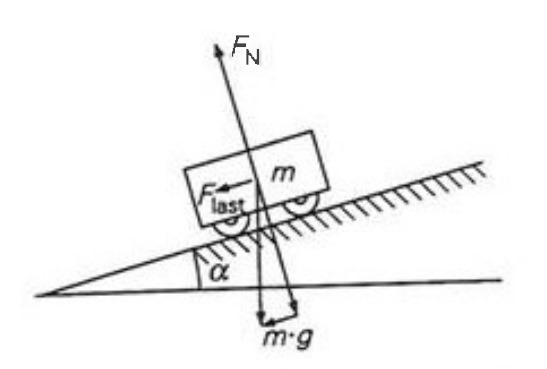
\includegraphics[scale=0.5]{Hellingsweerstand.jpg}
        \caption{hellinglast krachten}
    \end{figure}

    \begin{multicols}{2}
        \textbf{Formules:}
        \begin{equation}
            \begin{split}
                T_{last} &= f_{Z} \cdot sin(\alpha) \cdot r \\
                F_{Z} &= m \cdot g\\
                &\Downarrow \\
                T_{last} &= 2.43 \cdot sin(20) \cdot 0.075 = 62 [mNm]
            \end{split}
        \end{equation}

        \textbf{constante:}
        \begin{equation*}
            \begin{split}
                r &= 0,075 [m] \\
                m &= 1,5 [N] \\
                g &= 1,62 [m/s^2] \\
                \alpha &= 20^\circ 
            \end{split}
        \end{equation*}
    \end{multicols}

    \begin{figure}[H]
        \centering
        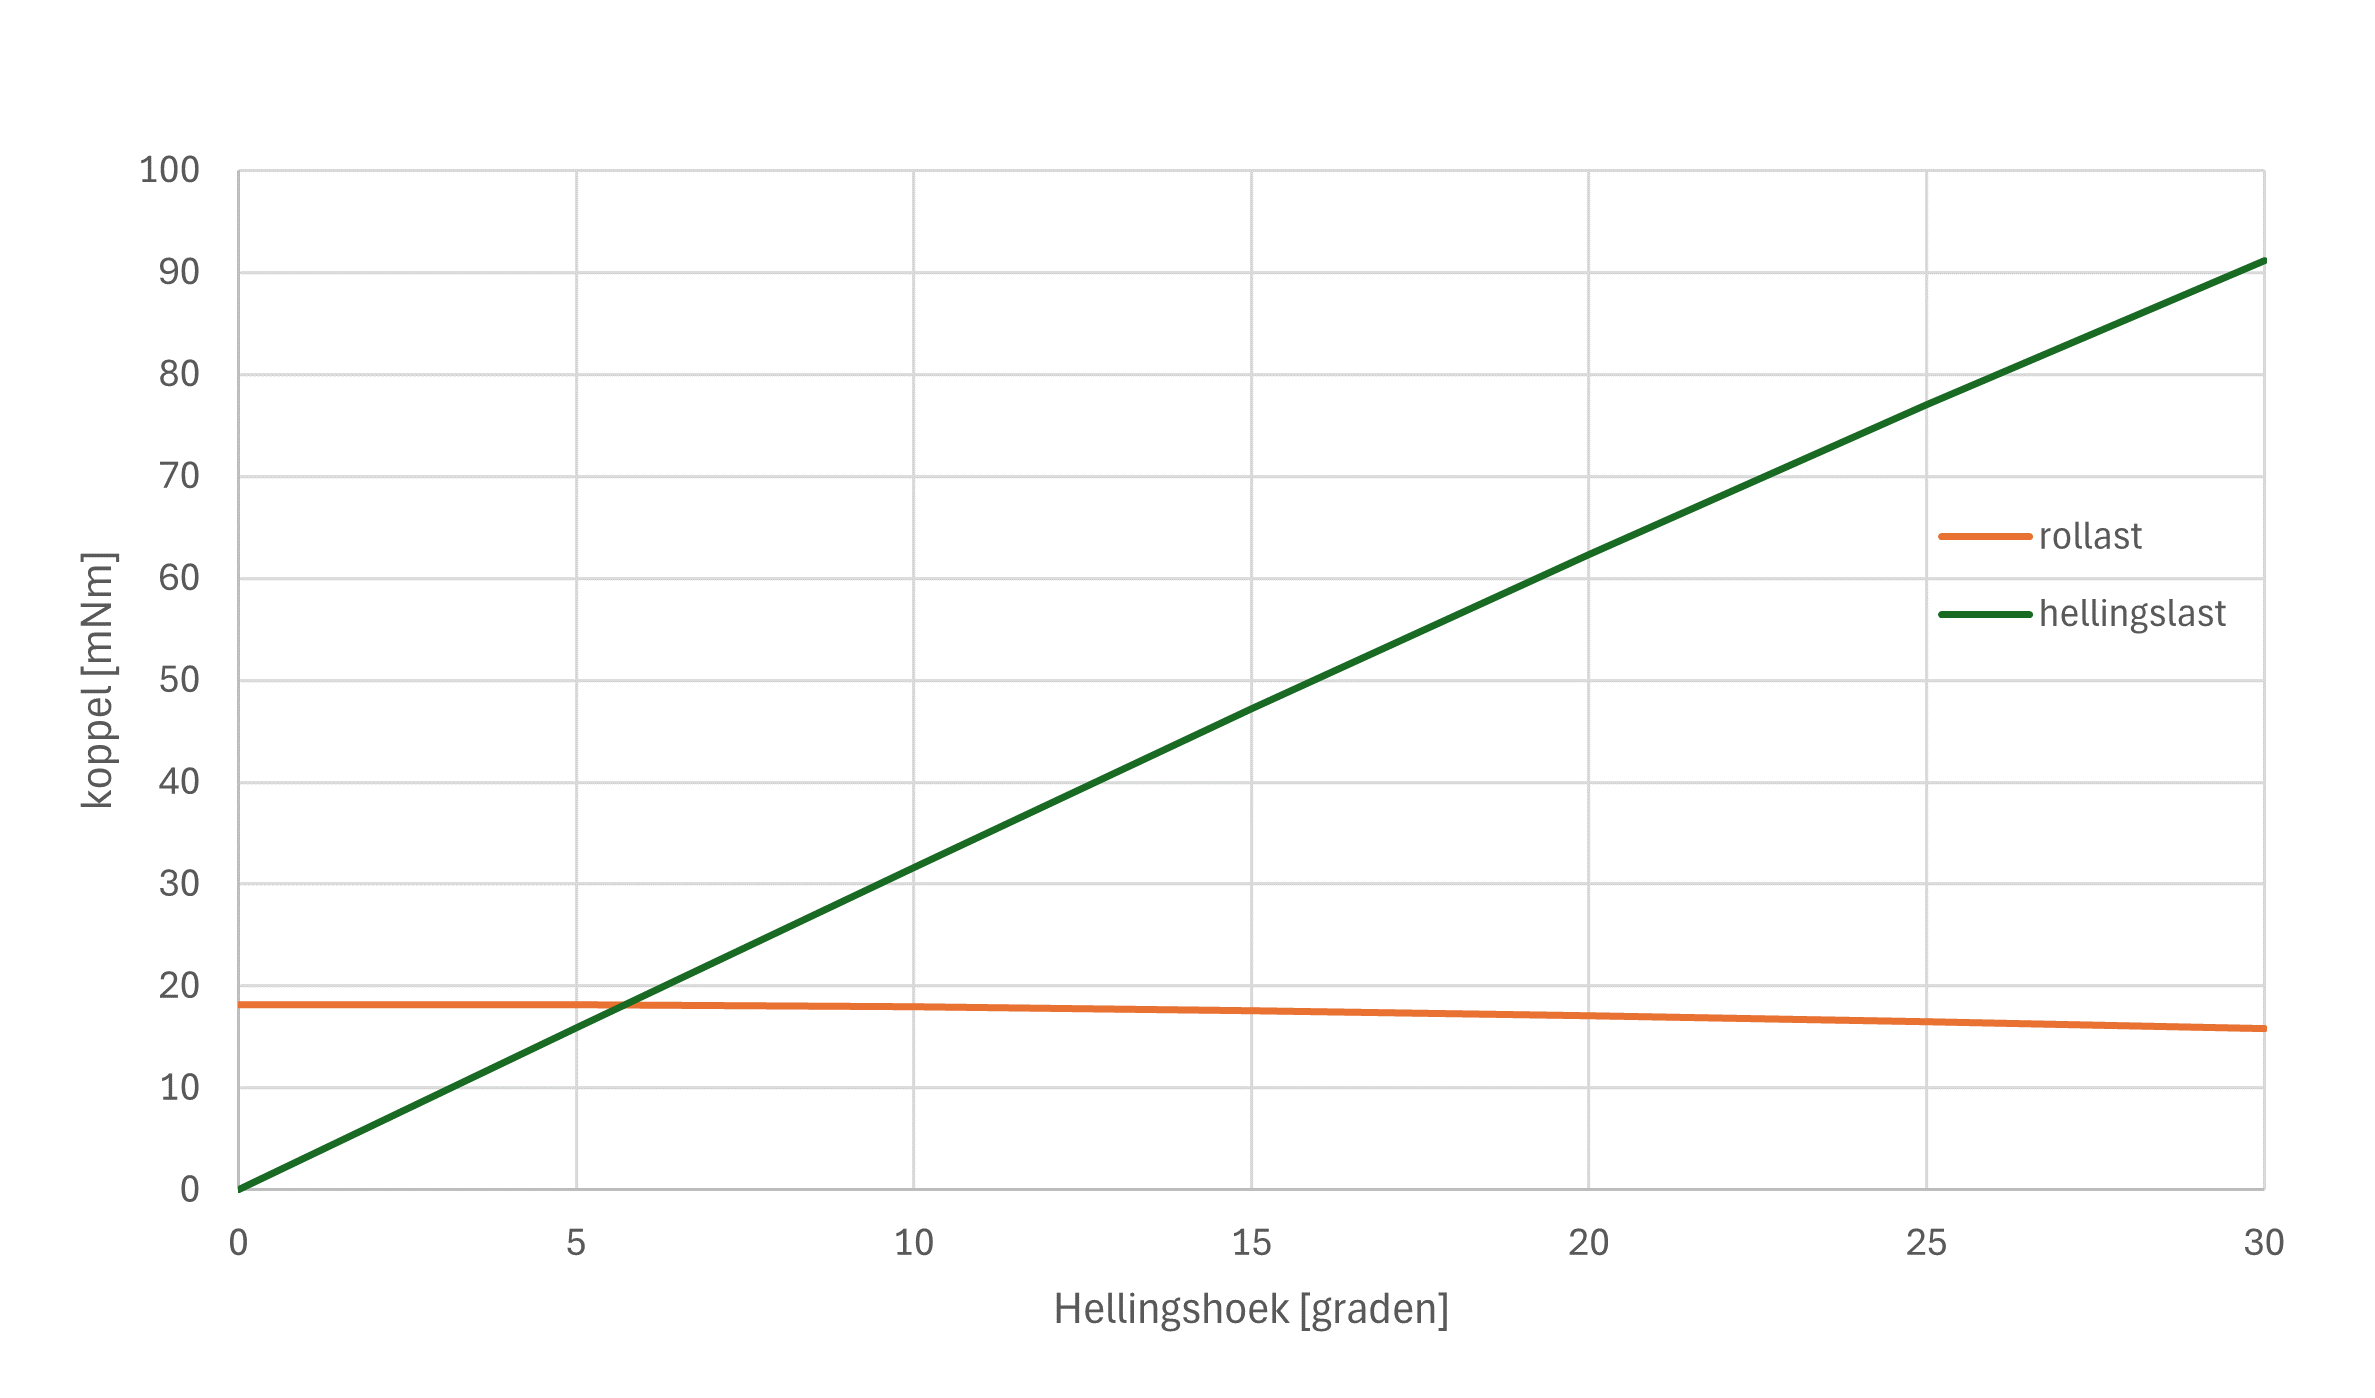
\includegraphics[scale=0.7]{rolkoppel_NEW.png}
        \caption{rollast vs hellingslast onder verschillende hoeken}
        \label{fig:birds}
    \end{figure}

    In figuur \ref{fig:birds} is te zien hoe de rolweerstand en de hellingsweerstand zich gedragen ten opzichte van verschillende hellingshoeken. In de grafiek is te zien dat vanaf een hoek van $5.72^\circ$ de moonrover altijd stil zal blijven staan. Dit komt doordat de moonrover tot dit punt nog niet voorbij zijn rollast komt. Het snijpunt van de rollast met de hellingslast word als volgt berekend:
    \begin{equation}
        \begin{split}
            T_{rollast} &= T_{hellingslast} \\
            f_{rol} \cdot F_{N} \cdot r &= F_{N} \cdot sin(\alpha) \cdot r \\
            f_{rol} &= sin(\alpha) \\
            0.1 &= sin(\alpha) \\
            \alpha &= sin-1(0.1) \\
            \alpha &= 5.72^\circ
        \end{split}
    \end{equation}

\subsection{Grip}
    Onder grip verstaan we de hoeveelheid koppel die op de aandrijving gegeven kan worden zonder dat het wiel zal gaan slippen. Hierbij berekenen we dus ook wat het maximale koppel is die gegeven kan worden op de aandrijving.

    \begin{multicols}{2}
        \textbf{Formules:}
        \begin{equation}
            \begin{split}
                T_{max} &= \mu \omega \cdot F_{N} \cdot r \\
                F_{N} &= m \cdot g \cdot cos(\alpha) \\
                &\Downarrow \\
                T_{max} &= 0.9 \cdot 2.43 \cdot 0.075 = 164.03 [mNm]
            \end{split}
        \end{equation}

        \textbf{constante:}
        \begin{equation*}
            \begin{split}
                \mu \omega &= 0.9 \\
                r &= 0,075 [m] \\
                m &= 1,5 [N] \\
                g &= 1,62 [m/s^2] \\
                \alpha &= 0^\circ 
            \end{split}
        \end{equation*}
    \end{multicols}

    \begin{figure}[H]
        \centering
        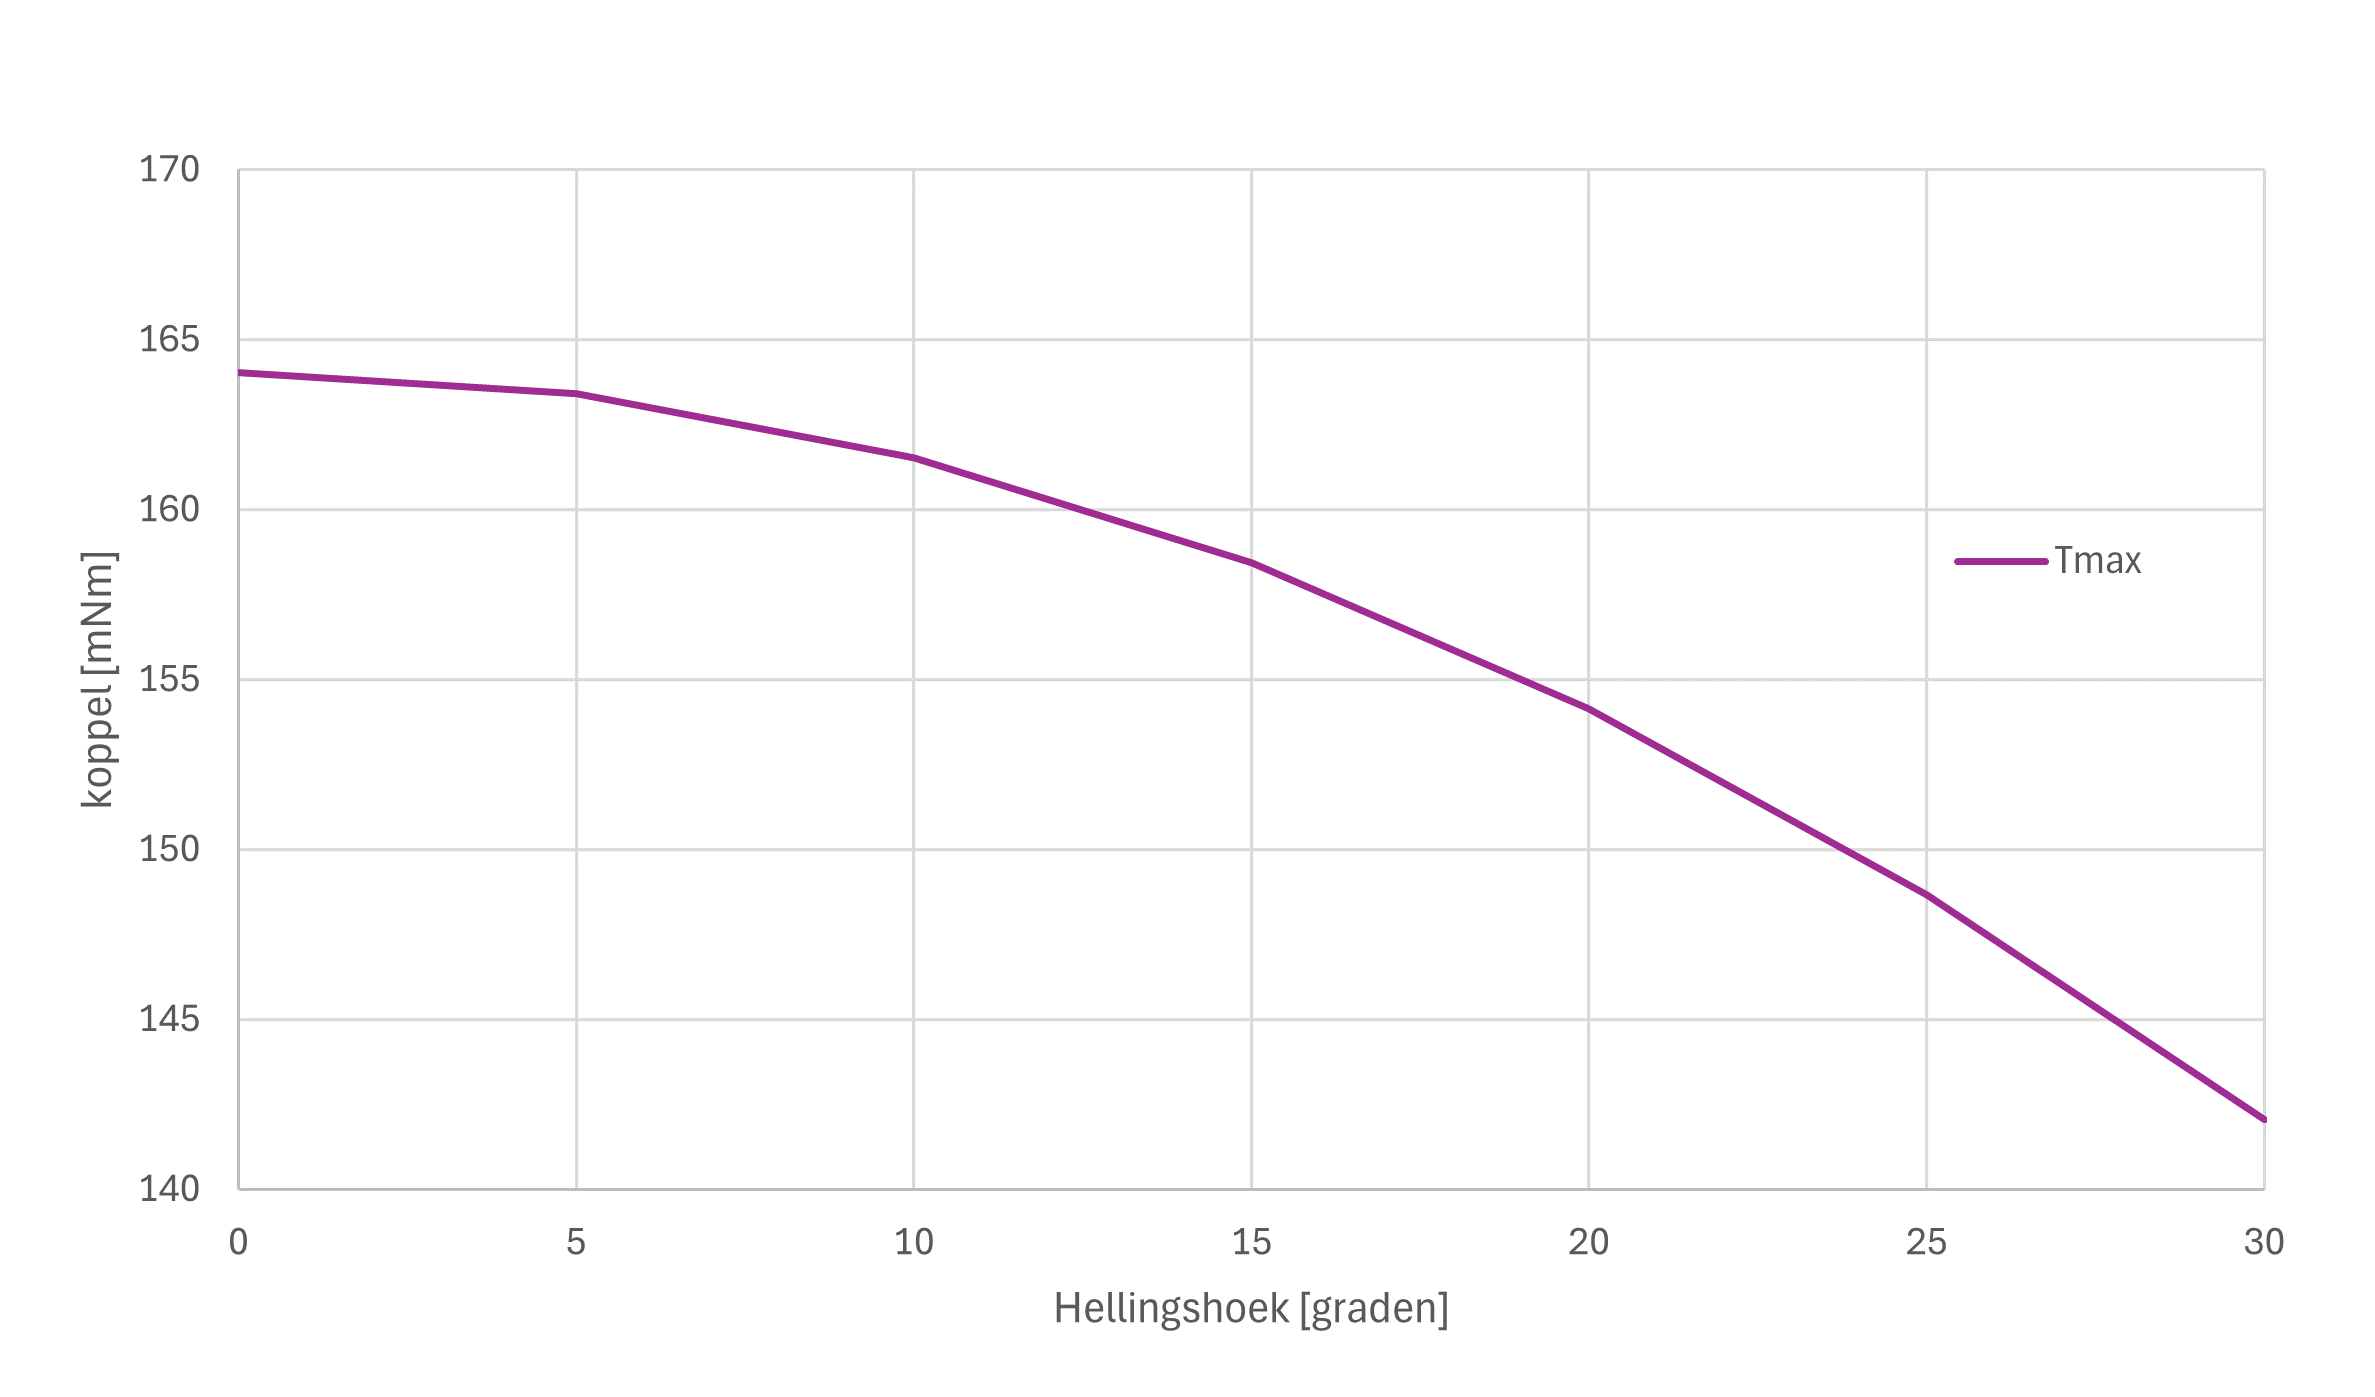
\includegraphics[scale=0.7]{maximumkoppel_NEW.png}
        \caption{$T_{max}$}
        \label{fig:peanut}
    \end{figure}

    In figuur \ref{fig:peanut} is te zien hoe de maximale koppel zich weerhoud tegen de hellingshoek. Hierbij is duidelijk te zien dat de maximale koppel afneemt naarmate de hellingshoek groter wordt.

\subsection{Versnelling}
    Hier word het koppeloverschot berekend wat nodig is om de beoogde versnelling te behalen voor het wiel; 

    \begin{multicols}{2}
        \textbf{Formules:}
        \begin{equation}
            \begin{split}
                T_{acc} &= J \cdot \frac{d \omega}{dt} \\
                omtrek_{wiel} &= 2 \cdot \pi \cdot r = 0.47 [m] \\
                Hoekversnelling &= \frac{a}{omtrek_{wiel}} = 1.49 [omwentelingen/s^2] \\
                &= 9.36 [rad/s^2] \\
                &\Downarrow \\
                T_{acc_{wiel}} &= 2.1 \cdot 10^{-3} \cdot 9.36 = 19.6 [mNm]\\
            \end{split}
        \end{equation}

        \textbf{constante:}
        \begin{equation*}
            \begin{split}
                a &= 0.7 [m/s^2] \\
                J &= 2.1 \cdot 10^{-3} [kg \cdot m^2]\\
                r &= 0,075 [m] \\
                g &= 1,62 [m/s^2] \\
                \alpha &= 0^\circ 
            \end{split}
        \end{equation*}
    \end{multicols}

Het koppel wat nodig is om het karretje te laten accelereren;

    \begin{multicols}{2}
        \textbf{Formules:}
        \begin{equation}
            \begin{split}
                F &= m \cdot a \\
                T_{acc_{karretje}} &= F \cdot r \\
                &\Downarrow \\
                T_{acc_{karretje}} &= 1,5 \cdot 0,7 \cdot 0,075 = 78,75 [mNm]
            \end{split}
        \end{equation}

        \textbf{constante:}
        \begin{equation*}
            \begin{split}
                a &= 0.7 [m/s^2] \\
                r &= 0.075 [m] \\
                m &= 1.5 [N] 
            \end{split}
        \end{equation*}
    \end{multicols}

Het koppel wat dan nodig is om het wiel en het karretje te laten accelereren is dan als volgt;

\begin{multicols}{2}
    \textbf{Formules:}
    \begin{equation}
        \begin{split}
            T_{acc_{totaal}} &= T_{acc_{wiel}} + T_{acc_{karretje}}\\
            &\Downarrow \\
            T_{acc_{totaal}} &= 19.6 + 78.75 = 98.35 [mNm]
        \end{split}
    \end{equation}

    \textbf{constante:}
    \begin{equation*}
        \begin{split}
            T_{acc_{wiel}} &= 19.6 [mNm] \\
            T_{acc_{karretje}} &= 78.75 [mNm] 
        \end{split}
    \end{equation*}
\end{multicols}

\subsection{Snelheid}
    Hier berekenen we de maximale rpm waarbij de maximale snelheid van van 2.1 m/s niet word overtroffen.

    \begin{multicols}{2}
        \textbf{Formules:}
        \begin{equation}
            \begin{split}
                omtrek &= 2 \cdot \pi \cdot r \\
                snelheid &= \frac{speed_{max}}{omtrek}\ = \frac{2.1}{0.47} = 4.46 [omw/s]\\
                &\Downarrow \\
                 &= 267.4 [rpm]
            \end{split}
        \end{equation}

        \textbf{constante:}
        \begin{equation*}
            \begin{split}
                speed_{max} &= 2.1 [m/s]\\
                r &= 0,075 [m] 
            \end{split}
        \end{equation*}
    \end{multicols}

\newpage

\subsection{Conclusie}
In dit hoofdstuk heb je kunnen lezen hoe we de lasten van de moonrover hebben bepaald. Dit was nodig om een geschikte motor te kunnen selecteren voor de moonrover.  In afbeelding \ref{fig:lasten moonrover} is het werkgebied te zien van de moonrover door middel van de rode lijnen. In het volgende hoofdstuk zal er een geschikte motor en transmissie geselecteerd worden die juist aansluit bij deze last. 

\begin{figure}[H]
    \centering
    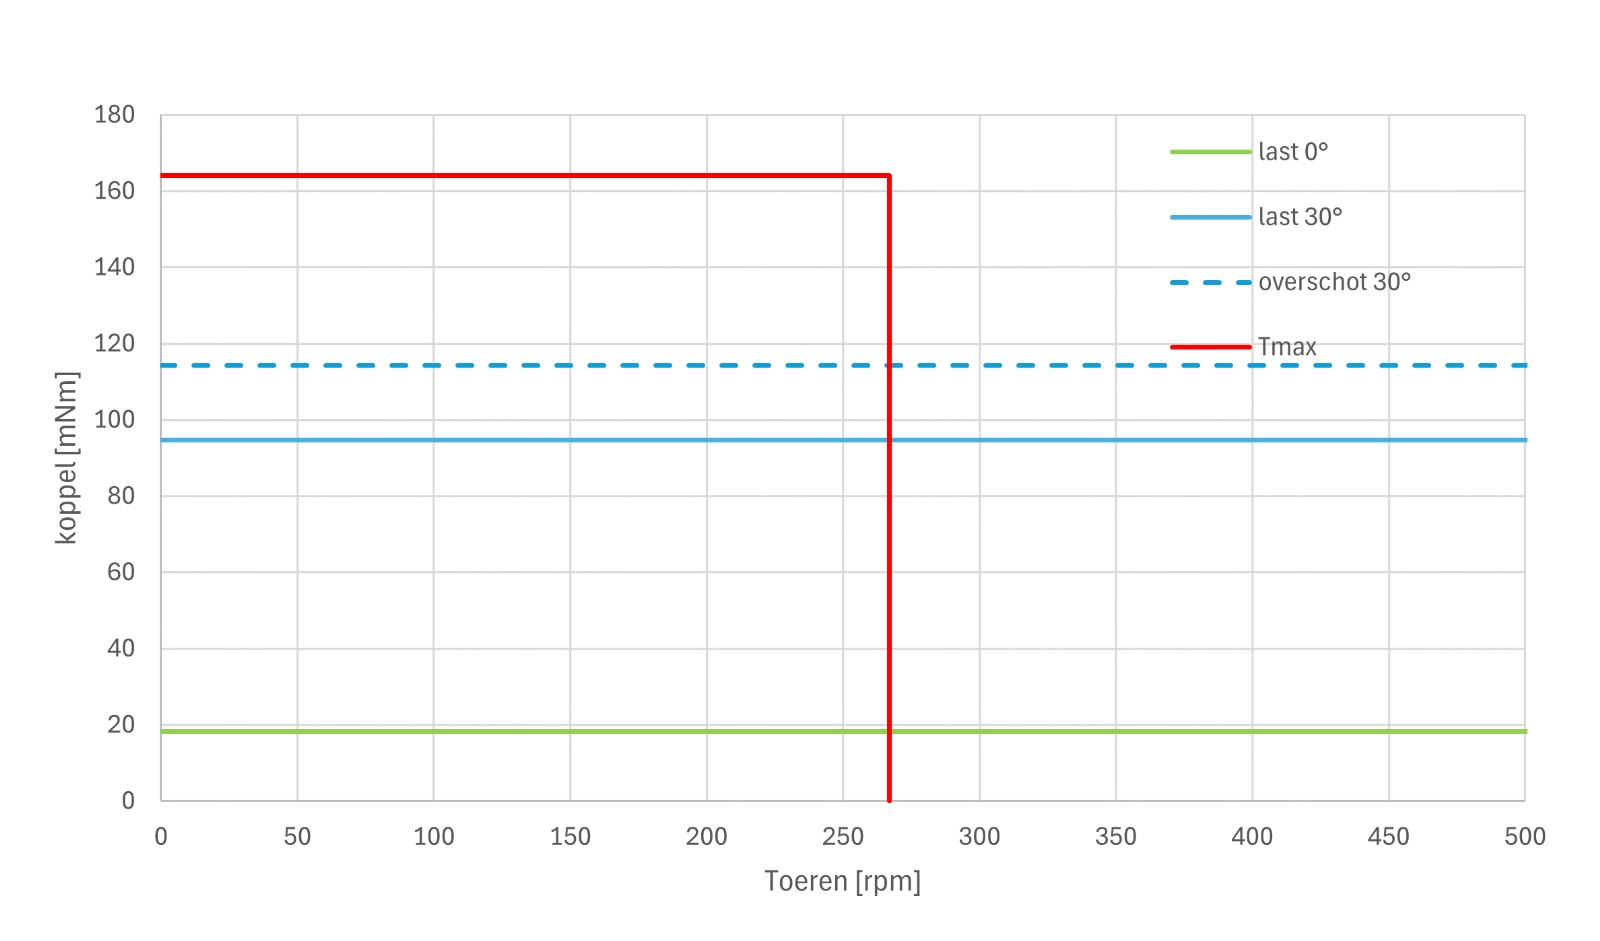
\includegraphics[scale=0.4]{last conclusie.jpg}
    \caption{Lasten moonrover}
    \label{fig:lasten moonrover}
\end{figure}
    
